\documentclass[journal]{vgtc}                % final (journal style)
%\documentclass[review,journal]{vgtc}         % review (journal style)
%\documentclass[widereview]{vgtc}             % wide-spaced review
%\documentclass[preprint,journal]{vgtc}       % preprint (journal style)

%% Uncomment one of the lines above depending on where your paper is
%% in the conference process. ``review'' and ``widereview'' are for review
%% submission, ``preprint'' is for pre-publication, and the final version
%% doesn't use a specific qualifier.

%% Please use one of the ``review'' options in combination with the
%% assigned online id (see below) ONLY if your paper uses a double blind
%% review process. Some conferences, like IEEE Vis and InfoVis, have NOT
%% in the past.

%% Please use the ``preprint''  option when producing a preprint version
%% for sharing your article on an open access repository

%% Please note that the use of figures other than the optional teaser is not permitted on the first page
%% of the journal version.  Figures should begin on the second page and be
%% in CMYK or Grey scale format, otherwise, colour shifting may occur
%% during the printing process.  Papers submitted with figures other than the optional teaser on the
%% first page will be refused. Also, the teaser figure should only have the
%% width of the abstract as the template enforces it.

%% These few lines make a distinction between latex and pdflatex calls and they
%% bring in essential packages for graphics and font handling.
%% Note that due to the \DeclareGraphicsExtensions{} call it is no longer necessary
%% to provide the the path and extension of a graphics file:
%% 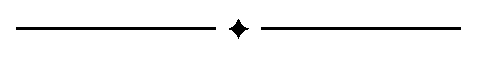
\includegraphics{diamondrule} is completely sufficient.
%%
\ifpdf%                                % if we use pdflatex
  \pdfoutput=1\relax                   % create PDFs from pdfLaTeX
  \pdfcompresslevel=9                  % PDF Compression
  \pdfoptionpdfminorversion=7          % create PDF 1.7
  \ExecuteOptions{pdftex}
  \usepackage{graphicx}                % allow us to embed graphics files
  \DeclareGraphicsExtensions{.pdf,.png,.jpg,.jpeg} % for pdflatex we expect .pdf, .png, or .jpg files
\else%                                 % else we use pure latex
  \ExecuteOptions{dvips}
  \usepackage{graphicx}                % allow us to embed graphics files
  \DeclareGraphicsExtensions{.eps}     % for pure latex we expect eps files
\fi%

%% it is recomended to use ``\autoref{sec:bla}'' instead of ``Fig.~\ref{sec:bla}''
\graphicspath{{figures/}{pictures/}{images/}{./}} % where to search for the images

\usepackage{microtype}                 % use micro-typography (slightly more compact, better to read)
\PassOptionsToPackage{warn}{textcomp}  % to address font issues with \textrightarrow
\usepackage{textcomp}                  % use better special symbols
\usepackage{mathptmx}                  % use matching math font
\usepackage{times}                     % we use Times as the main font
\renewcommand*\ttdefault{txtt}         % a nicer typewriter font
\usepackage{cite}                      % needed to automatically sort the references
\usepackage{tabu}                      % only used for the table example
\usepackage{booktabs}                  % only used for the table example
%% We encourage the use of mathptmx for consistent usage of times font
%% throughout the proceedings. However, if you encounter conflicts
%% with other math-related packages, you may want to disable it.

%% In preprint mode you may define your own headline. If not, the default IEEE copyright message will appear in preprint mode.
%\preprinttext{To appear in IEEE Transactions on Visualization and Computer Graphics.}

%% In preprint mode, this adds a link to the version of the paper on IEEEXplore
%% Uncomment this line when you produce a preprint version of the article 
%% after the article receives a DOI for the paper from IEEE
%\ieeedoi{xx.xxxx/TVCG.201x.xxxxxxx}

%% If you are submitting a paper to a conference for review with a double
%% blind reviewing process, please replace the value ``0'' below with your
%% OnlineID. Otherwise, you may safely leave it at ``0''.
\onlineid{0}

%% declare the category of your paper, only shown in review mode
\vgtccategory{Research}
%% please declare the paper type of your paper to help reviewers, only shown in review mode
%% choices:
%% * algorithm/technique
%% * application/design study
%% * evaluation
%% * system
%% * theory/model
\vgtcpapertype{Theory/Model}

%% Paper title.
\title{Topological Equivariance Artist Model}

%% This is how authors are specified in the journal style

%% indicate IEEE Member or Student Member in form indicated below
\author{A, B, C}
\authorfooter{
%% insert punctuation at end of each item
\item
 A B are with Computer Science, City College of New York. E-mail: roy.g.biv@aol.com.
\item
 Thomas Caswell is with Brookhaven National Lab E-mail: ed.grimley@aol.com.
}

%other entries to be set up for journal
\shortauthortitle{ \MakeLowercase{\textit{et al.}}: Topological Equivariant Artist Model}
%\shortauthortitle{Firstauthor \MakeLowercase{\textit{et al.}}: Paper Title}

%% Abstract section.
\abstract{ A critical aspect of data visualization is that the graphical representation of data is expected to match the properties of the data; this fails when order is not preserved in representations of ordinal data or scale for numerical data. In this work, we propose that the mathematical notions of equivariance and topology formalizes the expectation of matching properties. We developed a model we call the topological artist model (TAM) in which data and graphics can be viewed as sections of fiber bundles. This model allows for (1) decomposing the translation of data fields (variables) into visual channels via an equivariant map on the fibers and (2) a topology-preserving map of the base spaces that translates the dataset connectivity into graphical elements. Furthermore, our model supports an algebraic sum operation such that more complex visualizations can be built from simple ones. We illustrate the application of the model through case studies of a scatter plot, line plot, and heatmap. We show that this model can be implemented with a small prototype.} % end of abstract

%% Keywords that describe your work. Will show as 'Index Terms' in journal
%% please capitalize first letter and insert punctuation after last keyword
\keywords{Taxonomy, Models, Frameworks, Theory }

%% ACM Computing Classification System (CCS). 
%% See <http://www.acm.org/class/1998/> for details.
%% The ``\CCScat'' command takes four arguments.

\CCScatlist{ % not used in journal version
 \CCScat{K.6.1}{Management of Computing and Information Systems}%
{Project and People Management}{Life Cycle};
 \CCScat{K.7.m}{The Computing Profession}{Miscellaneous}{Ethics}
}

%% A teaser figure can be included as follows
\teaser{
  \centering
  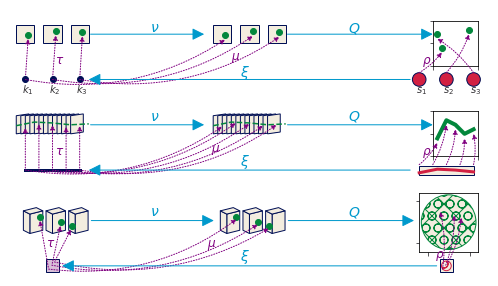
\includegraphics[width=\linewidth]{teaser.png}
  \caption{this is our model basically...}
  \label{fig:teaser}
}

%% Uncomment below to disable the manuscript note
%\renewcommand{\manuscriptnotetxt}{}

%% Copyright space is enabled by default as required by guidelines.
%% It is disabled by the 'review' option or via the following command:
% \nocopyrightspace


\vgtcinsertpkg

%%%%%%%%%%%%%%%%%%%%%%%%%%%%%%%%%%%%%%%%%%%%%%%%%%%%%%%%%%%%%%%%
%%%%%%%%%%%%%%%%%%%%%% START OF THE PAPER %%%%%%%%%%%%%%%%%%%%%%
%%%%%%%%%%%%%%%%%%%%%%%%%%%%%%%%%%%%%%%%%%%%%%%%%%%%%%%%%%%%%%%%%

\begin{document}

%% The ``\maketitle'' command must be the first command after the
%% ``\begin{document}'' command. It prepares and prints the title block.

%% the only exception to this rule is the \firstsection command
\firstsection{Introduction}
\maketitle
The aim of this work is to rearchitecture Matplotlib to take advantage of developments in software design, data structures, and visualization, 
to improve consistency, reusability, and discoverability, so that domain specific tool developers can build structure preserving visualization tools. We present a visualization model that formalizes constraints on componenents of a visualization in terms of equivaraiance, continuity, and composibility. 

\section{Background}
\begin{figure}[tb]
  \centering % avoid the use of \begin{center}...\end{center} and use \centering instead (more compact)
  \includegraphics[width=\columnwidth]{paper-count-w-2015-new}
  \caption{A visualization of the 1990--2015 data from \autoref{tab:vis_papers}. The image is from \cite{Isenberg:2017:VMC} and is in the public domain.}
  \label{fig:sample}
 \end{figure}

\section{Model}

\section{Prototype}

\begin{figure}[tb]
 \centering % avoid the use of \begin{center}...\end{center} and use \centering instead (more compact)
 \includegraphics[width=\columnwidth]{paper-count-w-2015-new}
 \caption{A visualization of the 1990--2015 data from \autoref{tab:vis_papers}. The image is from \cite{Isenberg:2017:VMC} and is in the public domain.}
 \label{fig:sample}
\end{figure}

\subsubsection{Ejector Seat Reservation}

Duis autem~\cite{Lorensen:1987:MCA}\footnote{The algorithm behind
Marching Cubes \cite{Lorensen:1987:MCA} had already been
described by Wyvill et al. \cite{Wyvill:1986:DSS} a year
earlier.} vel eum iriure dolor in hendrerit
in vulputate velit esse molestie consequat,\footnote{Footnotes
appear at the bottom of the column.} vel illum dolore eu
feugiat nulla facilisis at vero eros et accumsan et iusto odio
dignissim qui blandit praesent luptatum zzril delenit augue duis
dolore te feugait nulla facilisi. Lorem ipsum dolor sit amet,
consectetuer adipiscing elit, sed diam nonummy nibh euismod tincidunt
ut laoreet dolore magna aliquam erat volutpat.


\paragraph{Confirmed Ejector Seat Reservation}

Ut wisi enim ad minim veniam, quis nostrud exerci tation ullamcorper
suscipit lobortis nisl ut aliquip ex ea commodo
consequat~\cite{Nielson:1991:TAD}. Duis autem vel eum iriure dolor in
hendrerit in vulputate velit esse molestie consequat, vel illum dolore
eu feugiat nulla facilisis at vero eros et accumsan et iusto odio
dignissim qui blandit praesent luptatum zzril delenit augue duis
dolore te feugait nulla facilisi.

\paragraph{Rejected Ejector Seat Reservation}

Ut wisi enim ad minim veniam, quis nostrud exerci tation ullamcorper
suscipit lobortis nisl ut aliquip ex ea commodo consequat. Duis autem
vel eum iriure dolor in hendrerit in vulputate velit esse molestie

\subsection{Vestibulum}

Vestibulum ut est libero. Suspendisse non libero id massa congue egestas nec at ligula. Donec nibh lorem, ornare et odio eu, cursus accumsan felis. Pellentesque habitant morbi tristique senectus et netus et malesuada fames ac turpis egestas. Donec dapibus quam vel eros mattis, id ornare dolor convallis. Donec at nisl sapien. Integer fringilla laoreet tempor. Fusce accumsan ante vel augue euismod, sit amet maximus turpis mattis. Nam accumsan vestibulum rhoncus. Aenean quis pellentesque augue. Suspendisse sed augue et velit consequat bibendum id nec est. Quisque erat purus, ullamcorper ut ex vel, dapibus dignissim erat.

Quisque sit amet orci quam. Lorem ipsum dolor sit amet, consectetur adipiscing elit. Aliquam pharetra, nunc non efficitur convallis, tellus purus iaculis lorem, nec ultricies dolor ligula in metus. Class aptent taciti sociosqu ad litora torquent per conubia nostra, per inceptos himenaeos. Aenean eu ex nulla. Morbi id ex interdum, scelerisque lorem nec, iaculis dui. Phasellus ultricies nunc vitae quam fringilla laoreet. Quisque sed dolor at sem vestibulum fringilla nec ac augue. Ut consequat, velit ac mattis ornare, eros arcu pellentesque erat, non ultricies libero metus nec mi. Sed eget elit sed quam malesuada viverra. Quisque ullamcorper, felis ut convallis fermentum, purus ligula varius ligula, sit amet tempor neque dui non neque. Donec vulputate ultricies tortor in mollis.

Integer sit amet dolor sit amet turpis ullamcorper varius. Cras volutpat bibendum scelerisque. Maecenas mauris dolor, gravida eu elit et, sodales consequat tortor. Integer id commodo elit. Pellentesque sollicitudin ex non nulla molestie eleifend. Mauris sagittis metus nec turpis imperdiet, vel ullamcorper nibh tincidunt. Sed semper tempus ex, ut aliquet erat hendrerit id. Maecenas sit amet dolor sollicitudin, luctus nunc sit amet, malesuada justo.

Mauris ut sapien non ipsum imperdiet sodales sit amet ac diam. Nulla vel convallis est. Etiam dapibus augue urna. Aenean enim leo, fermentum quis pulvinar at, ultrices quis enim. Sed placerat porta libero et feugiat. Phasellus ullamcorper, felis id porta sollicitudin, dolor dui venenatis augue, vel fringilla risus massa non risus. Maecenas ut nulla vitae ligula pharetra feugiat non eu ante. Donec quis neque quis lorem cursus pretium ac vulputate quam. Cras viverra tellus vitae sapien pretium laoreet. Pellentesque fringilla odio venenatis ex viverra, quis eleifend tortor ornare. Ut ut enim nunc. Vivamus id ligula nec est dignissim eleifend.

Nunc ac velit tellus. Donec et venenatis mauris. Lorem ipsum dolor sit amet, consectetur adipiscing elit. Ut vitae lectus vel ante mollis congue. Vestibulum at cursus velit. Curabitur in facilisis enim. Vestibulum eget dui aliquet risus laoreet laoreet. Phasellus et est id magna interdum venenatis. Donec luctus vehicula justo sed laoreet. Quisque tincidunt suscipit augue, in molestie sem accumsan sed.
\section{Conclusion}

Lorem ipsum dolor sit amet, consetetur sadipscing elitr, sed diam
nonumy eirmod tempor invidunt ut labore et dolore magna aliquyam erat,
sed diam voluptua. At vero eos et accusam et justo duo dolores et ea
rebum. Stet clita kasd gubergren, no sea takimata sanctus est Lorem
ipsum dolor sit amet. Lorem ipsum dolor sit amet, consetetur
sadipscing elitr, sed diam nonumy eirmod tempor invidunt ut labore et
dolore magna aliquyam erat, sed diam voluptua. At vero eos et accusam
et justo duo dolores et ea rebum. Stet clita kasd gubergren, no sea
takimata sanctus est Lorem ipsum dolor sit amet. Lorem ipsum dolor sit
amet, consetetur sadipscing elitr, sed diam nonumy eirmod tempor
invidunt ut labore et dolore magna aliquyam erat, sed diam
voluptua. At vero eos et accusam et justo duo dolores et ea
rebum.


%% if specified like this the section will be committed in review mode
\acknowledgments{
The authors wish to thank A, B, and C. This work was supported in part by
a grant from XYZ (\# 12345-67890).}

%\bibliographystyle{abbrv}
\bibliographystyle{abbrv-doi}
%\bibliographystyle{abbrv-doi-narrow}
%\bibliographystyle{abbrv-doi-hyperref}
%\bibliographystyle{abbrv-doi-hyperref-narrow}

\bibliography{template}
\end{document}

